%\documentclass[paper]{geophysics}
\documentclass[manuscript,revised]{geophysics}


% An example of defining macros
\newcommand{\rs}[1]{\mathstrut\mbox{\scriptsize\rm #1}}
\newcommand{\rr}[1]{\mbox{\rm #1}}

\newcommand{\psm}{\textit{PSM} }
\newcommand{\twod}{two-dimensional }
\newcommand{\thrd}{three-dimensional }

\usepackage{lineno}

% printing options
%\usepackage{pgfpages}
%\pgfpagesuselayout{4 on 1}[letterpaper,border shrink=5mm]


\begin{document}

\title{tmp title: MUSC source}

\renewcommand{\thefootnote}{\fnsymbol{footnote}} 

\ms{GEO-Example} % manuscript number

\address{
\footnotemark[1]LUNAM-IFSTTAR, \\
\footnotemark[2]OSUNA \\
\footnotemark[1]LPGN, \\}
\author{Damien Pageot\footnotemark[1]\footnotemark[2], Donatienne Leparoux\footnotemark[1], Mathieu Le Feuvre\footnotemark[1], Olivier Durand\footnotemark[1] and Yann Capdeville\footnotemark[3]}

\footer{Example}
\lefthead{Dellinger \& Fomel}
\righthead{\emph{Geophysics} example}

\maketitle

\begin{abstract}
\end{abstract}

\modulolinenumbers[5]
\linenumbers

% ## INTRODUCTION
\section{Introduction}
      
\noindent Since the early developments of seismic imaging methods in the middle of 20th century, approaches and algorithms innovations are still proposed in current research projects. The improvements deal with both the qualitative imaging techniques like migration (e.g. \citet{Berkhout_MSS_2012,Guofeng_GPU_2013}), novel applications of quantitative imaging methods such as the first arrival tomography (e.g. \citet{Bohm_CWS_2015}), or even more recent approaches like the Full Waveform Inversion (e.g. \citet{Perez_AWI_2014}, see \citet{Virieux_FWI_2009} for a revue of this last decade). The refinements are proposed for different scales like near surface applications for civil engineering topics or more deeper investigation for example for oil prospection or crustal imaging at regional or global scales They are mostly validated by using synthetic data, for example with well known shared benchmark (like the Marmousi case). However, the synthetic data are generally computed using the same wave propagation modeling engine used in the inverse problem process. In other terms, the synthetic data are computed with some assumptions which are the same in the inverse problem, for example the approximation of acoustic propagation, a 2D space medium, or a 2D line source. This aproach, called \textit{inverse crime} \citep{Wirgin_TIC_2004} is particularly useful for validating an algorithm in its early development stage but does not take into account the artefacts that can be due to the assumptions of the direct problem. Some authors tackle this issue by providing 3D data which are inverted with a 2D approach or other restrictive assumptions (e.g ). But also in this case, the approach does not allow to assess the efficiency of the method for real seismic data. Moreover, because no one knows precisely the Earth interior, it is difficult to evaluate the capacity of a method to recover physical parameters and structures from real seismic data which can lead sometimes to geological misinterpretation due to numerical artifacts \citep{Morozov_ARF_2004}. Thus, it is necessary to add a step for which imaging methods will be tested for experimental seismic measurements obtained under controlled conditions.
	
\noindent The best way to satisfy this need is to use Physical Small Scale Modeling Methods (noted \psm subsequently). \psm were used since several years to study the propagation of waves in various media with several stage of complexity, from acoustic wave propagation in homogeneous media to elastic wave propagation in \thrd heterogeneous anisotropic media \citep{Rieber_EWP_1936,Howes_SMS_1953,Hilterman_TDM_1970,French_MRP_1974,Bishop_LVM_1985,Pratt_FWI_1999,Favretto_NMT_2013,Sarkar_TPM_2003,Isaac_SMS_1999}, and allow to generate experimental seismic data under well-controlled conditions. In this way, recent studies have been conducted to simulate multi-sources and multi-receivers through piezzo-electric transducers \citep{Wong_SPM_2009}. An alternative approach consists in using the laser interferometry as the receiver system, as done in the MUSC Laboratory \citep{Bretaudeau_SSA_2008b,Bretaudeau_SSM_2011,Bretaudeau_FWI_2013}, \textit{Mesure Ultrasonore Sans Contact} in French, is one of them. This technology, by avoiding the contact of the receivers on the model, allows to by-pass the coupling issue of transducers that is difficult to model. In this way,the MUSC laboratory is designed to simulate (1) wide-angle on-shore acquisitions modeling both body waves and surface waves, (2) automatic multisource-multireceiver measurements with a high-productivity, (3) high-precision source-receiver positioning and (4) high-precision recording of absolute surface displacement without coupling effects. 
	
% #### State the objectives
\noindent Our objective here is to increase the potential of the MUSC system as a reliable tool for generating experimental data which will be distributed in the scientific community. 
\noindent Thus, we present two studies of experimental data in order to : 1) refine the comparison between numerical and experimental data by taking into account the 3D/2D geometrical spreading effects through an alternative way and 2) identify the reproducibility of the source impact and, consequently, data repeatability. These approaches will complete the knowledge of the system and facilitate the achievement of massive multi-source and multi-receiver data simulating subsurface seismic experimental campaigns.
	
% #### Describe the method of investigation
\noindent To achieve some of these objectives, we used a seismic wave modeling code based on the Spectral Element Method \citep{Komatitsch_SEM_1998,Komatitsch_ISM_1999,Komatitsch_SEM_2005,Festa_PML_2005}. This method has several advantages compared to finite differences and finite elements, such as: (1) a weak formulation which can naturally take into account the free surface, (2) an explicit scheme in time facilitating parallelization and reducing the computational cost, (3) a spatial discretization (mesh) convenient for the representation of complex environments and (4) high precision results and low numerical dispersion.
	
% #### Describe the principal results of the investigation
	
\noindent Thus, this article is organized as follow. In a first part, we present he MUSC laboratory and the SEM code used for the studies. In a second part, we present two coupled studies of experimental data in order to: (1) refine the comparison between numerical and experimental data by taking into account the geometrical spreading effects between \twod and \thrd data through an alternative way, and (2) identify the reproducibility of the source impact to validate the data reproducibility.


% ## METHODS
\section{Methods}

% #### MUSC bench
\subsection{Physical modeling: MUSC system}

\noindent The MUSC system \citep{Bretaudeau_SSA_2008b,Bretaudeau_SSM_2011,Bretaudeau_FWI_2013} is built to experimentally reproduce field seismic data with a great accuracy on small scale model. Figure \ref{panel_musc_bench} shows the bench and its components. MUSC system is composed of a honeycomb tab and two arms which control the source and the receiver position with a precision of 10 $\mathrm{\mu m}$.

\noindent The receiving system of MUSC system is a laser interferometer. The principle of this laser is based on a phase shift of the reflected laser signal due to the wave propagation in the material. A real-time calibration value enables a continuous conversion to a nanometric displacement. The focal diameter of the laser on the model surface is about several micrometers and allows a detection limit of $\mathrm{2.5\ nm}$ (few) in the frequency range from 30 kHz to 20 MHz.

\noindent The seismic source is simulated by a piezoelectric transducer relied to a launching and synchronization system. This system provides more energy than a laser impulse source \citep{Bretaudeau_PHD_2010,Bretaudeau_SSM_2011} and allows to choose the source function, \textit{i.e.}, Gauss source, Ricker source, central frequency $f_{0}$ and time delay $t_{0}$. The source is generated by a waveform generator and is then amplified before transmitted to the small-scale-model. In the framework of seismic physical modeling, the source must be as closed as possible to a normal point source. Thus, the piezoelectric source is coupled with an adapter in order to reproduce the spatial energy repartition (limiting directivity) and conserving the waveform as shown in figure \ref{piezo-source-validation}.

\noindent For the purpose of small scale modeling, the change of scale must keep the relationship between observables. For most of seismic imaging methods, the significant physical parameters are the compressional and shear waves velocities, $V_{P}$ and $V_{S}$ respectively, the density $\rho$ and the quality factor $Q$. When scaling the model, many parameters can be modified: the distances, the time scale, the amplitudes of the signals, the viscoelastic properties, etc. Hence, the predominant factor is the wavelength $\lambda = V / f$, where $V$ is the wave velocity and $f$ the frequency. Thus, physical and mechanical parameters are modified to preserve the ratio $\lambda_{real} = \xi \lambda_{scale}$ where $\xi$ is the scale ratio. It is therefore necessary to act directly on the time-frequency scales. Assuming the materials used to build the small scale model have the same mechanical properties ($V_{P}$, $V_{S}$, $\rho$) than the natural media, it is straightforward to obtain the scale ratios for parameters involved in seismic experiment.

\noindent For near surface experiments, the scale ratio $\xi$ is about $1000$ which means that the central frequency $f_{0}$ of the source is few $kHz$ (generally 100 kHz but can be more or less), distances are in $mm$ (acquisition length around 50 mm typically) and time unit is $ms$.( $V_{P}$, $V_{S}$ etc...)

\noindent Small-scale models are generally made of metal, thermoplastic or melted epoxy resin-based materials \citep{Bretaudeau_FWI_2013,Bretaudeau_SSM_2011,Bretaudeau_SSA_2008b}. These materials allow to reproduce complex geometries and have a large panel of physical and mechanical properties. These materials have the advantages to have physical properties closed to natural soil materials after scaling. The models are generally over-sized to easily separate reflected waves on boundaries from the rest of the signal. 

% #### Spectral Element Method
\subsection{Numerical modeling: Spectral Element Method}

\noindent Various numerical methods exist to resolve the equation of motion in arbitrary elastic media. The most widely used is the Finite-Differences (FD) method \citep{Virieux_PSV_1986,Levander_PSV_1988,Robertsson_FDM_1994,Pratt_EWM_1990,Stekl_VEM_1998,Saenger_FDM_2004} which estimates each derivative on a regular Cartesian grid using a Taylor development \citep{Moczo_FDM_2004} of order \textit{n}. FD is simple to implement but quickly shows some limitations: the Cartesian grid is defined by the minimum propagated wavelength ($\lambda_{min}$) in the full media and is unable to reproduce properly complex topography and interfaces. Moreover, \citet{Saenger_FDM_2000} show that 60 points by wavelength ($\lambda$) are needed to model propagation of Rayleigh wave in order $n=2$ where only 15 points by $\lambda$ are required to model propagation of body waves which increases drastically the numerical cost in case of near-surface modeling experiment. The Finite-Elements Method (FEM) is another popular method used for wave propagation modeling \citep{Lysmer_FEM_1972,Seron_FEM_1990,Hulbert_FEM_1990}. FEM is based on a variational formulation of the equation of motion and gives a continuous approximate solution in space using polynomial basis functions defined on each node of each cell of the mesh. The natural boundary conditions of FEM is the free surface and the triangular (in 2D) or tetraedric (in 3D) unstructured meshes are well adapted to complex media and topography. However, low polynomial basis are inadequate with fine spatial discretization and the required discretization to obtain precise and non-dispersive solution is numerically costly. 

\noindent Recently, the Spectral Element Method (SEM), widely used in fluid dynamics \citep{Patera_SEM_1984,Korczak_SEM_1986,Karniadakis_FEM_1989}, was adapted to seismic wave propagation \citep{Komatitsch_SEM_1998,Komatitsch_ISM_1999,Komatitsch_SEM_2005,Festa_PML_2005}. 

\noindent The SEM is based upon a high-order piecewise polynomial approximation of the weak formulation of the wave equation. It combines the accuracy of the pseudo-spectral method with the flexibility of the finite-element method \citep{Tromp_SEM_2008}. 

\noindent In this method, the wave-field is represented in terms of high-degree Lagrange interpolants, and integrals are computed based upon Gauss-Lobatto-Legendre (gll) quadrature. This combination leading to a perfectly diagonal mass matrix leads in turn to a fully explicit time scheme which leads itself very well to numerical simulations on parallel computers. It is particularly well suited to handling complex geometries and interface matching conditions \citep{Cristini_SEM_2012}. 

\noindent As in FEM, all boundary of the domain are reflecting and the free surface is the natural condition.  In order to simulate infinite or semi-infinite domain, SEM can use Perfect Match Layers boundary conditions \citep{Berenger_PML_1994,Festa_PML_2005} but are not used here.
 
\noindent The typical element size that is required to generate an accurate mesh is of the order of $\lambda$, $\lambda$ being the smallest wavelength of waves traveling in the model.

\noindent Models are meshed in 2D with quadrangles using the open-source software package GMSH \citep{Geuzaine_MSH_2009}. 

% ## Models
\section{Models}

% ## Results
\section{Results}

% #### From point-source to line-source acquisition
\subsection{From point-source to line-source response}

\noindent In the framework of wave propagation modeling and imaging methods, most of available algorithms are limited to the \twod approximation especially for computational cost causes. More, a widely used way to validate imaging methods consists in inverse crime while the validity of applications on real dataset is conditioned by strong \textit{a priori} and a weak knowledge of the target. All of these leads to a limited validation of the efficiency imaging methods to recover parameter models. Thus, it is critical for 2D inversion of field date to accurately correct the geometrical spreading.

\noindent Point-source data can corrected from geometrical spreading using a simple two-steps signal processing: (1) convolving each trace by $\sqrt{t^{-1}}$, where $t$ is the time, to correct the phase shift of $\pi/4$ (2) applying a taper $\sqrt{t}$ to all traces to correct amplitudes. Some variation exist, for examples, using a linear source wavelet estimation method to correct the phase \citep{Bretaudeau_FWI_2013} or applying an offset conditioning \citep{Tran_SWT_2013}. To correct some biases of these methods, \citet{Forbriger_LSS_2014} and \citet{Schafer_LSS_2014} have introduced, and successfully applied to synthetic data, the \textit{hybrid method}. In the \textit{hybrid method} the geometrical spreading correction is conditioned by: (1) the offset, (2) the knowledge of the wave propagation velocities in the medium and (3) a user defined ratio used to smoothly correct amplitudes from near to far offsets. The results are thus strongly dependent of user's \textit{a priori} and attempts. However, this kind of signal corrections are valid only for two-dimensional ($x,z$) medias invariant along the $y$-axis.    

\noindent In other cases, 3D data are corrected or process \textit{on the fly}, or used as is in algorithm using a 2.5D approximation.

\noindent Thus, the missing step between purely numerical validation and real data applications can be the use of experimental line-source seismograms recorded under controlled conditions.

\noindent Here, we take advantage of the experimental framework to explore an alternative approach specific to MUSC system. Figure \ref{amplitude_acqui_principle} presents a schematic representation of the principle for this kind of experiment. Theoretically, the stack of all receiver with the same offset will results in a pseudo line-source response. Yet, to simplify the experiment, an other way is to consider only one receiver per offset, on a line perpendicular  and centered to the defined line-source. All traces of each common receiver gather are then stacked together to obtain the line-source response. In order to apply this protocol, we have to choose a line-source's length $L$ sufficiently great to be assimilated to a cylindrical source and above all a suitable sampling interval $\Delta s$ between each point-source constituting the pseudo line-source to ensure applicability of the \textit{Huygen's principle}. 

\noindent For this experiment, we choose an homogeneous block of \textit{F50 pure} epoxy-resin (see table \ref{epoxy-resin} for physical parameters) with dimensions $500 \times 504 \times 115$ mm ($x \times y \times z$). Given the material's properties, we choose $L=240\ mm$ and $ds=0.5\ mm$ which leads to 481 point-source locations. Four receiver positions have been selected: 45, 50, 55 and 60 mm offset perpendicular to the line-source. The source wavelet is a Ricker with a central frequency $f_{0}=100\ kHz$.Each receiver is perpendicular to and centered on the line-source. For each receiver position, all recorded traces are stacked together to obtain an equivalent two-dimensional line-source response.

\noindent We first apply this method using 2D and 3D numerical modeling for 3D point-source, 3D line-source and 2D cylindrical source with a complete acquisition of 120 receivers spaced of 1 mm and a minimum offset of 45 mm. For these experiments, we did not take into account the quality factor $\mathcal{Q}$. Figure \ref{panel_amplitude_sem}a shows the comparison between point-source response (3D) and line-source response (2D). As expected, both amplitude and phase are differents. Then, we applied the \textit{hybrid method} \citep{Forbriger_LSS_2014;Schafer_LSS_2014} on the point-source response to obtain the equivalent line-source response. Figure \ref{panel_amplitude_sem}b shows that the \textit{hybird method} is able to produce equivalent line-source response with a good agreement.

\noindent To evaluate the efficiency of the method, experimental line-source responses will be compared to point-source and equivalent line-source responses using the cross-correlation coefficient (\textbf{cc}) and the root mean square (\textbf{rms}) ratio. These values are presented in table \ref{cc-rms}. \textbf{cc}$_init$ and \textbf{rms}$_init$ correspond to direct evaluation whereas \textbf{cc}$_final$ corresponds to the best \textbf{cc} obtained and \textbf{rms}$_final$ is the corresponding \textbf{rms}.

\noindent We now apply this method to experimental data on the equivalent real reduced-scale model. Figures \ref{panel_amplitude}(a) show the comparison between experimental traces obtained using a point-source and a line-source for source-receiver offsets 50, 55, 60 and 65 mm respectively. It is straightforward that these waveforms are not similar in terms of both phases (\textbf{cc}$<$0.75) and amplitude (\textbf{rms}$>$0.4). Even after amplitude fitting, point-source response to the line-response in term of phase (\textbf{cc}$<$0.8), amplitudes do not match (\textbf{rms}$>$0.4). These results confirm that using raw point-source responses in a \twod inversion process or imaging method can be critical in terms of convergence and validity of the results since these methods are built over phase and/or amplitude similarity.

\noindent Figures \ref{panel_amplitude}(b) show the comparison between experimental traces using a line-source and a point-source after geometrical spreading corrections (equivalent line-source response) using the same parameters than for numerical experiment. The cross-correlation coefficient \textbf{cc} for these waveforms are greater than 0.95 and rms$<$0.25. These results denote that the experimental line-source response is correct in terms of phase compared to an equivalent line-source response. However, \textbf{rms} are quite great even if they are smaller than previously. This can be explained by small differences in terms of waveforms and phases which are critical in the final \textbf{rms} results. Moreover, the \textit{hybrid} method to obtain the equivalent line-source response from a point-source response needs accurate parametrization to obtain the best result which is not necessarily in a good agreement with the attempt true line-source response.   

\noindent These results show that the line-source emulation on the MUSC system is efficient and can produce data suitable for imaging methods such as 2D FWI.


% #### Experimental source reproducibility
\subsection{Experimental source reproducibility}

\noindent We have shown the MUSC system is able to generate high quality 2D experimental seismograms. However, experimental data, as other, must be reproducible to be used as a reference or in an inversion process. As shown by \citet{Bretaudeau_SSM_2011}, the source waveform injected in the reduced-scale model by the piezo-electric source is not similar to the selected theoritical one. Figure (?), of data recorded in an homogeneous model, shows clearly multiple wavefront following the main arrival. After \citet{Bretaudeau_SSM_2011}, these multiples are generated inside the conical adapter of the piezo-electric source.

\noindent To assess the ability of MUSC system to provide reproducible data, \textit{i.e.} to evaluate the reproducibility of the source impact, several physical modeling were performed on the same homogeneous epoxy-resin block as in previous section. 

\noindent Ten realizations have been acquired on this model with a similar geometry setup, i.e. 120 receivers positions with an increment equal to 1 mm and a minimum offset of 10 mm. The numerical wavelet sent to the piezoelectric transducer source is a Ricker signal with a central frequency of 100 kHz. However, the source waveform is modified by the physical coupling effect of the transducer. 

\noindent A mean shot gather, calculated from the ten experiments, is used as reference seismogram. Figure \ref{panel_central_traces_cc} shows the central trace of each realization and \textbf{cc} gives the correlation coefficient of each trace with the reference one. The \textbf{cc} are always greater than 0.98 which demonstrate the very high reproducibility of data generated by the MUSC system.

\noindent In a second step, a unique source wavelet is estimated using a linear source wavelet estimation method based on a stabilized deconvolution \citep{Pratt_FWI_1999}. The source wavelet estimation takes into account the ten experiments together and allows to obtain a mean effective source suitable for each experiment. The resulting source wavelet is applied to the synthetic signals (figure \ref{panel_srcest_2d_mean_comp}). The corrected seismograms are in good agreement with the experimental seismograms (correlation coefficients $\mathrm{>}$ 0.96) confirms the great efficiency of the wavelet source assessment process.  

\noindent These last results, based on an average estimated source wavelet show that the effective impulse source emitted by the transducer in the MUSC system measurement bench is stable enough to ensure a robust reproducibility of the source. Therefore, concerning the key issue of the source knowledge, experimental data acquired in the MUSC system can be efficiently processed by imaging methods like Full Waveform Inversion (FWI) with only one estimation step for all the multi-source and multi-receivers data.

\noindent However, this last result does not mean that the source will be the same for an experiment for an other experiment on an other model. Thus, we consider now a more complex model, called \textit{BiAlt}. This model , shown in figure (???) is a two-layer model with a central alteration. We generate synthetic seismogram with the 2D SEM algorithm and using the mean effective source wavelet estimated on homogeneous block as a source function. Figure \ref{blind-test} shows that the synthetic seismogram using the effective source wavelet is in good agreement with the experimental one...

\noindent This last result shows that the MUSC source is stable from an experiment to an other and can be consequently injected as an input in modeling and imaging methods without any pre-processing or \textit{on the fly} source inversion.

% ## CONCLUSIONS

\section{Conclusions}

\noindent These two studies allow to refine the capacity of the physical modeling designed for seismic experiments simulation by 1) completing the validation of the measurement through comparison of numerical and experimental data generated by a realistic 2D source line and 2) assessing the reproductivity of the effective source emitted in a model. These improvements allow to provide and distribute experimental reduced scale data to the scientific community as benchmark datasets.

% ## PLOTS
\section{Plots}

\subsection*{Equations}

\subsection*{Figures}

% #### Fig:: panel_musc_bench
\begin{figure}[!h]
	\centering
	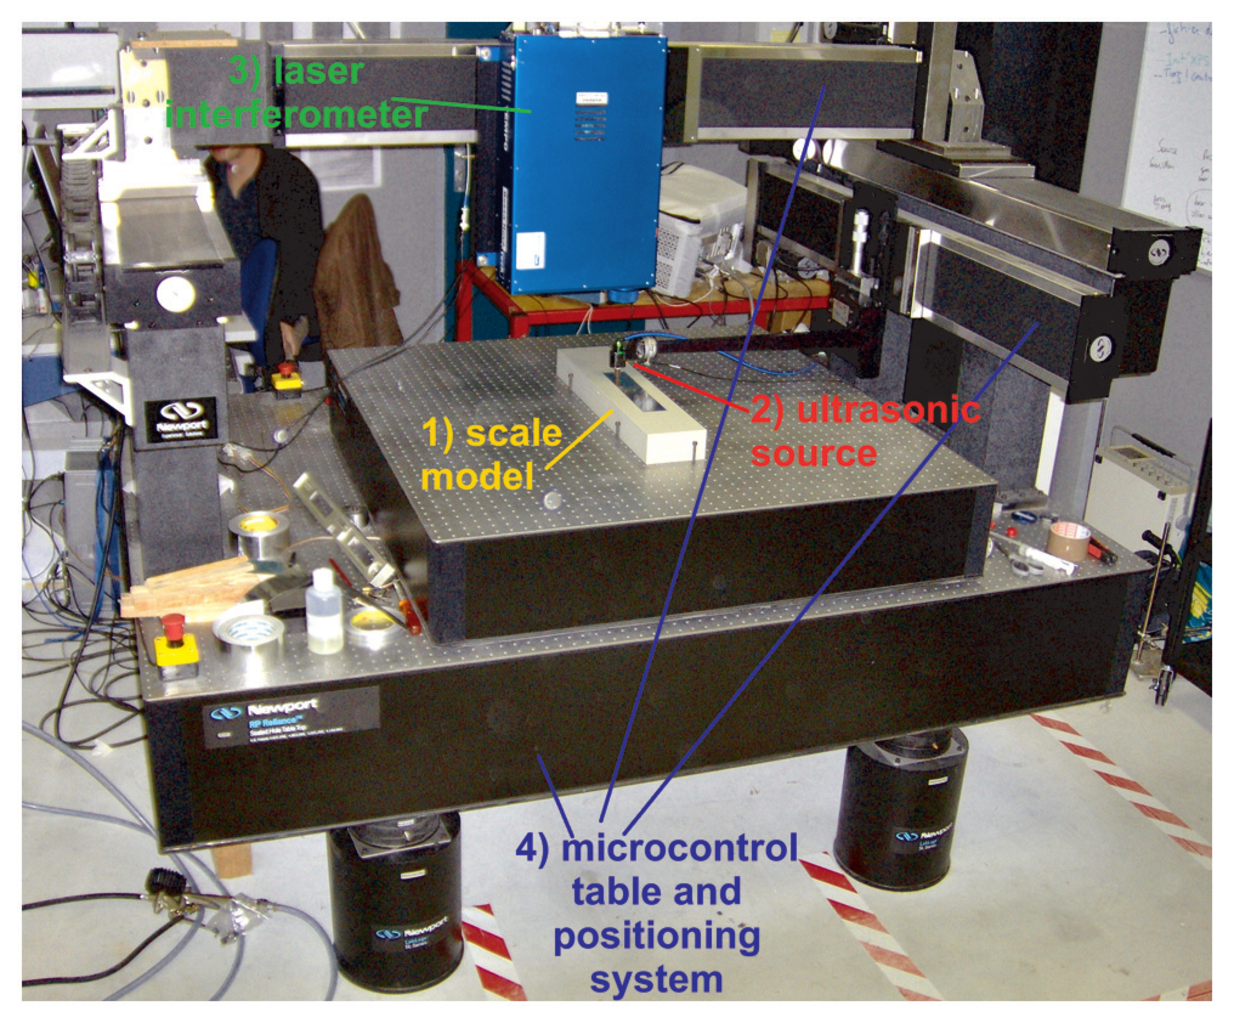
\includegraphics[scale=0.5]{fig/panel_musc_bench.eps}
	\caption{Photograph of the MUSC ultrasonic laboratory (from \citet{Bretaudeau_FWI_2013} )with its four components: (1) a small-scale model of the underground, (2) an optical table with two automated arms moving above the model, (3) a laser interferometer recording ultrasonic wave propagation	at the model surface, and (4) a piezoelectric ultrasonic source generating ultrasonic waves in the model.}
	\label{panel_musc_bench}
\end{figure}

% #### Fig:: panl_multisrcrec
\begin{figure}[!h]
	\centering
	\includegraphics[scale=0.5]{fig/panel_multisrcrec.eps}
	\caption{Example of multi-source multi-receiver record on the MUSC system for a two-layer model (bialt).}
	\label{panel_multisrcrec}
\end{figure}

% #### Fig:: piezo-source-validation
\begin{figure}[!ht]
	\centering
	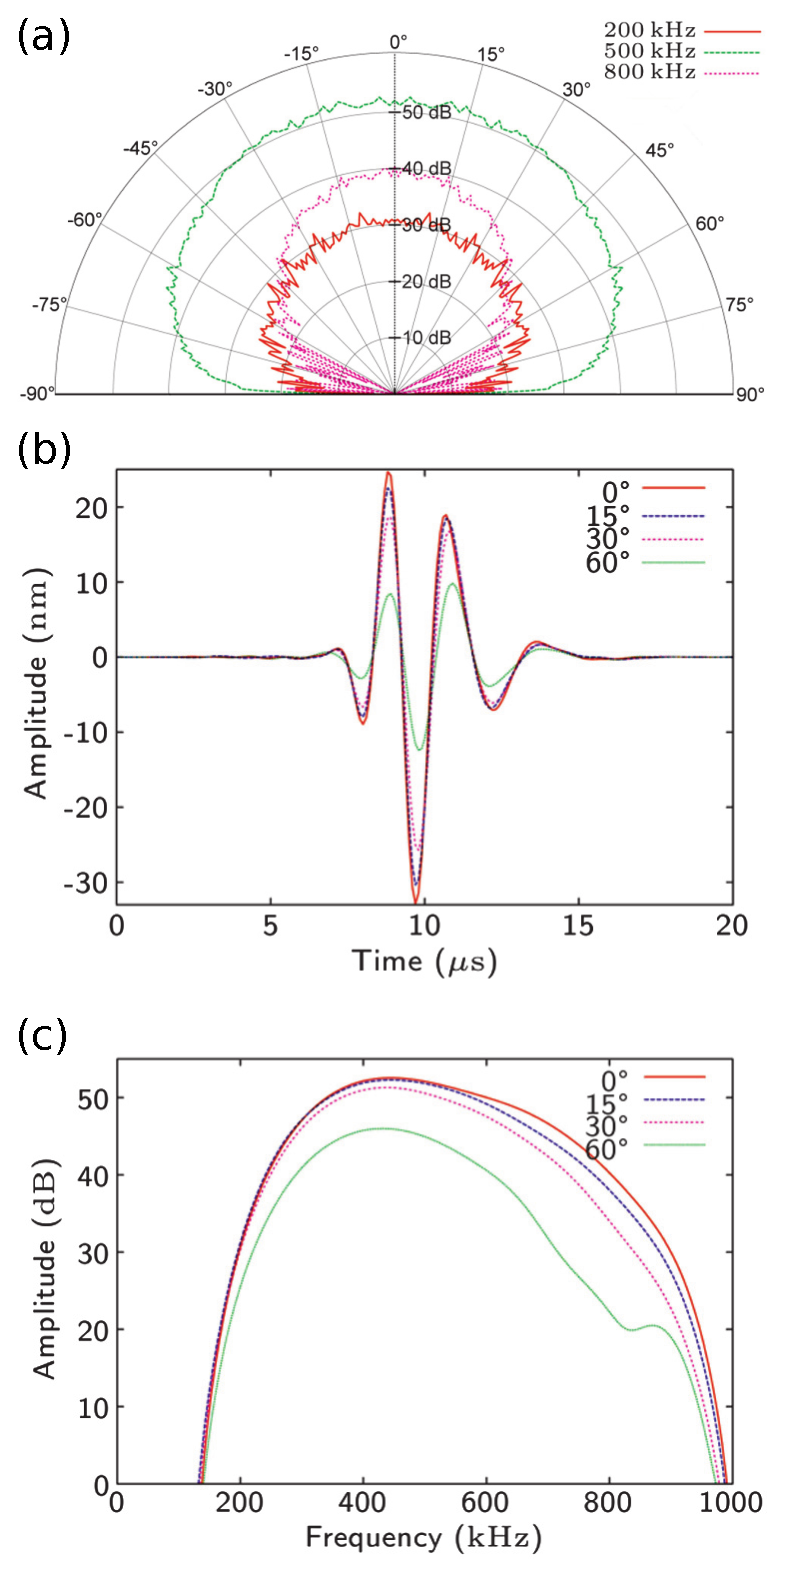
\includegraphics[scale=0.5]{fig/piezo-source-validation.eps}
	\caption{Validation of the piezoelectric source coupled with an adapter \citep{Bretaudeau_SSM_2011}. (a) Directivity diagrams (dB) for the high-frequency source Panametrics\textregistered with conical polyurethane adapter: three frequencies — normal particle displacement. (b) Temporal signals and (c) amplitude spectrums for the high-frequency source Panametrics\textregistered with a conical polyurethane adapter in transmission through a PVC cylinder for	various angles of incidence: O, 15, 30, and 60 degrees — normal particle displacement.}
	\label{piezo-source-validation}
\end{figure}

% #### Fig:: panel_bialt_2d3d
\begin{figure}[!h]
	\centering
	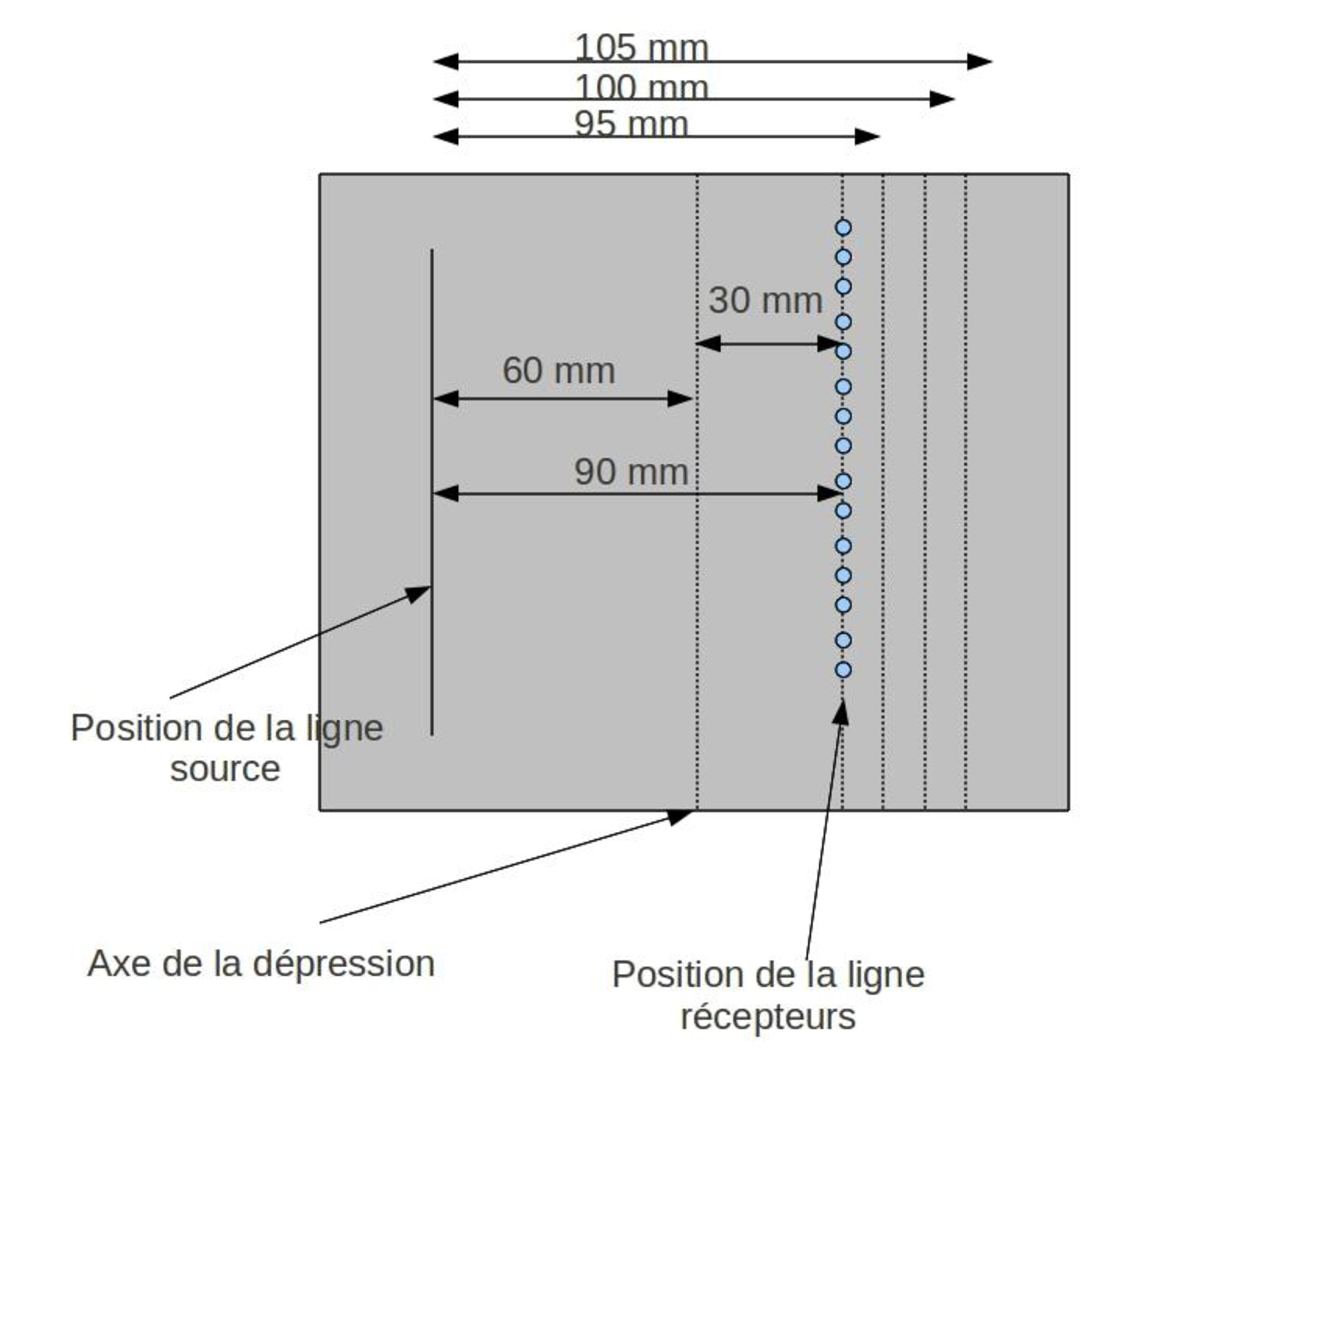
\includegraphics[scale=0.5]{fig/amplitude_acqui_principle.eps}
	\caption{Schematic representation of the acquisition geometry used to generate experimental line-source, \textit{i.e.} an equivalent of cylindrical source use in two-dimensional modeling. Black traingle and red circle represent receivers and sources, respectively.}
	\label{amplitude_acqui_principle}
\end{figure}

\begin{figure}[!h]
	\centering
	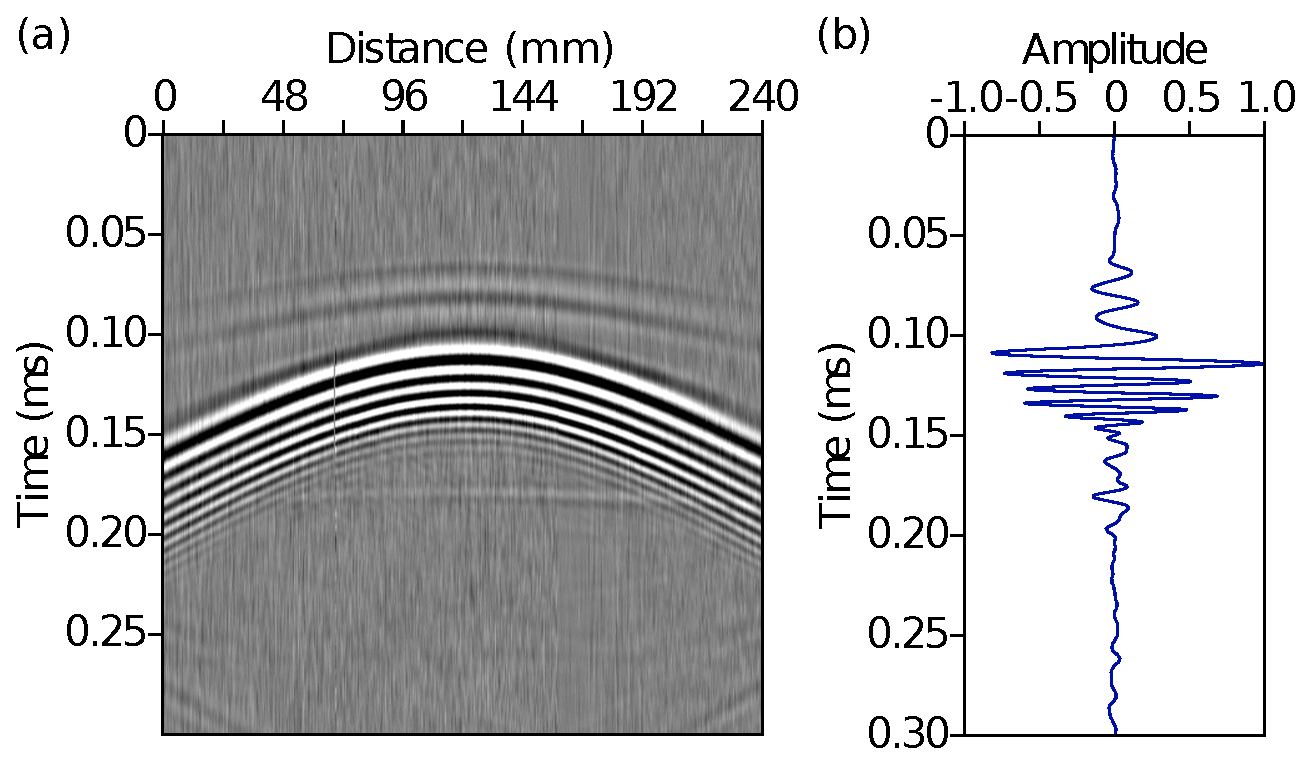
\includegraphics[scale=0.5]{fig/amplitude_stack_principle.eps}
	\caption{(a) Resulting seismogram at one receiver position for the experimental line-source. (b) Comparison between point-source response in red (central trace of (a)) and line-source response in green (stack of (a)). Some wavefront are pointed: (1) P-wave, (2) surface wave, (3) reflected \textit{PP} and (4) reflected \textit{PSv} -wave on the bottom of the model.}
	\label{amplitude_stack_principle}
\end{figure}

\begin{figure}[!h]
	\centering
	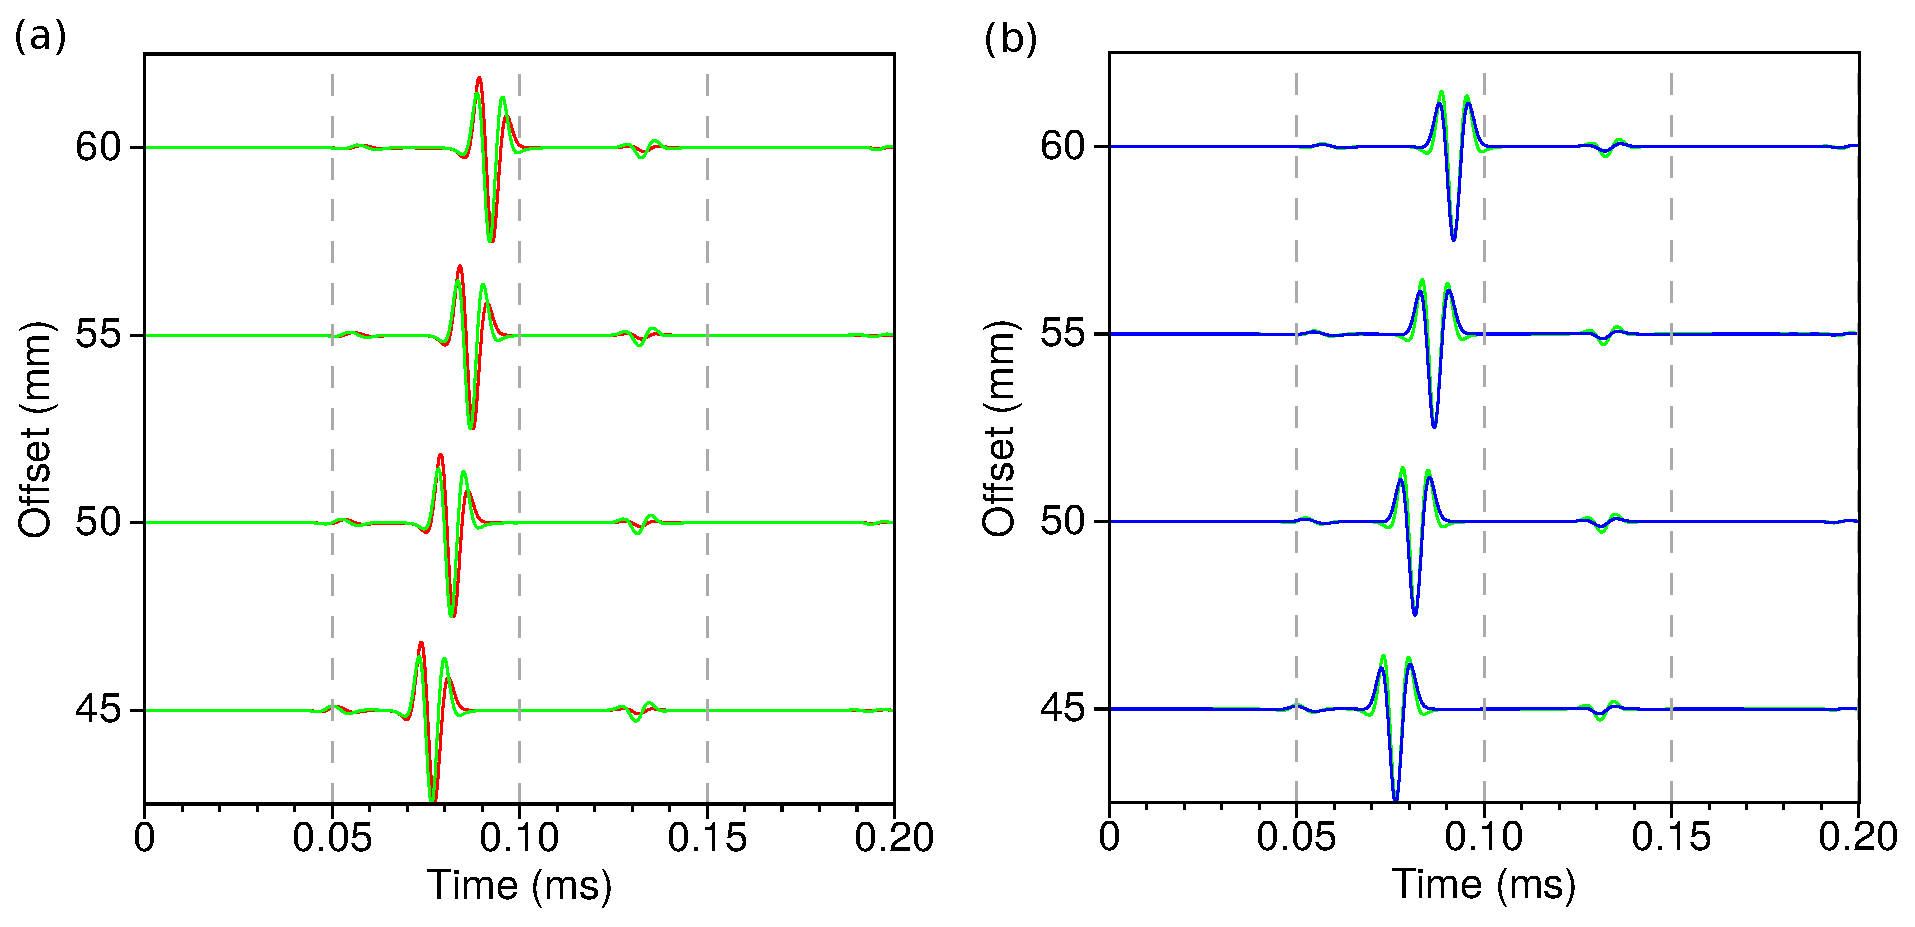
\includegraphics[scale=0.5]{fig/trans2d3d.eps}
	\caption{(a) Comparison between an experimental seismogram for a point-source (red) and for a line source (black), for 50, 55, 60 and 65 mm source-receiver offsets respectively. (b) Comparison between an experimental seismogram for a line-source (black), and a point-source response corrected from geometrical spreading (green) for same source-receiver offsets as (a). \textbf{cc} gives the correlation factor between line-source and point-source responses.}
	\label{panel_amplitude_sem}
\end{figure}

\begin{figure}[!h]
	\centering
	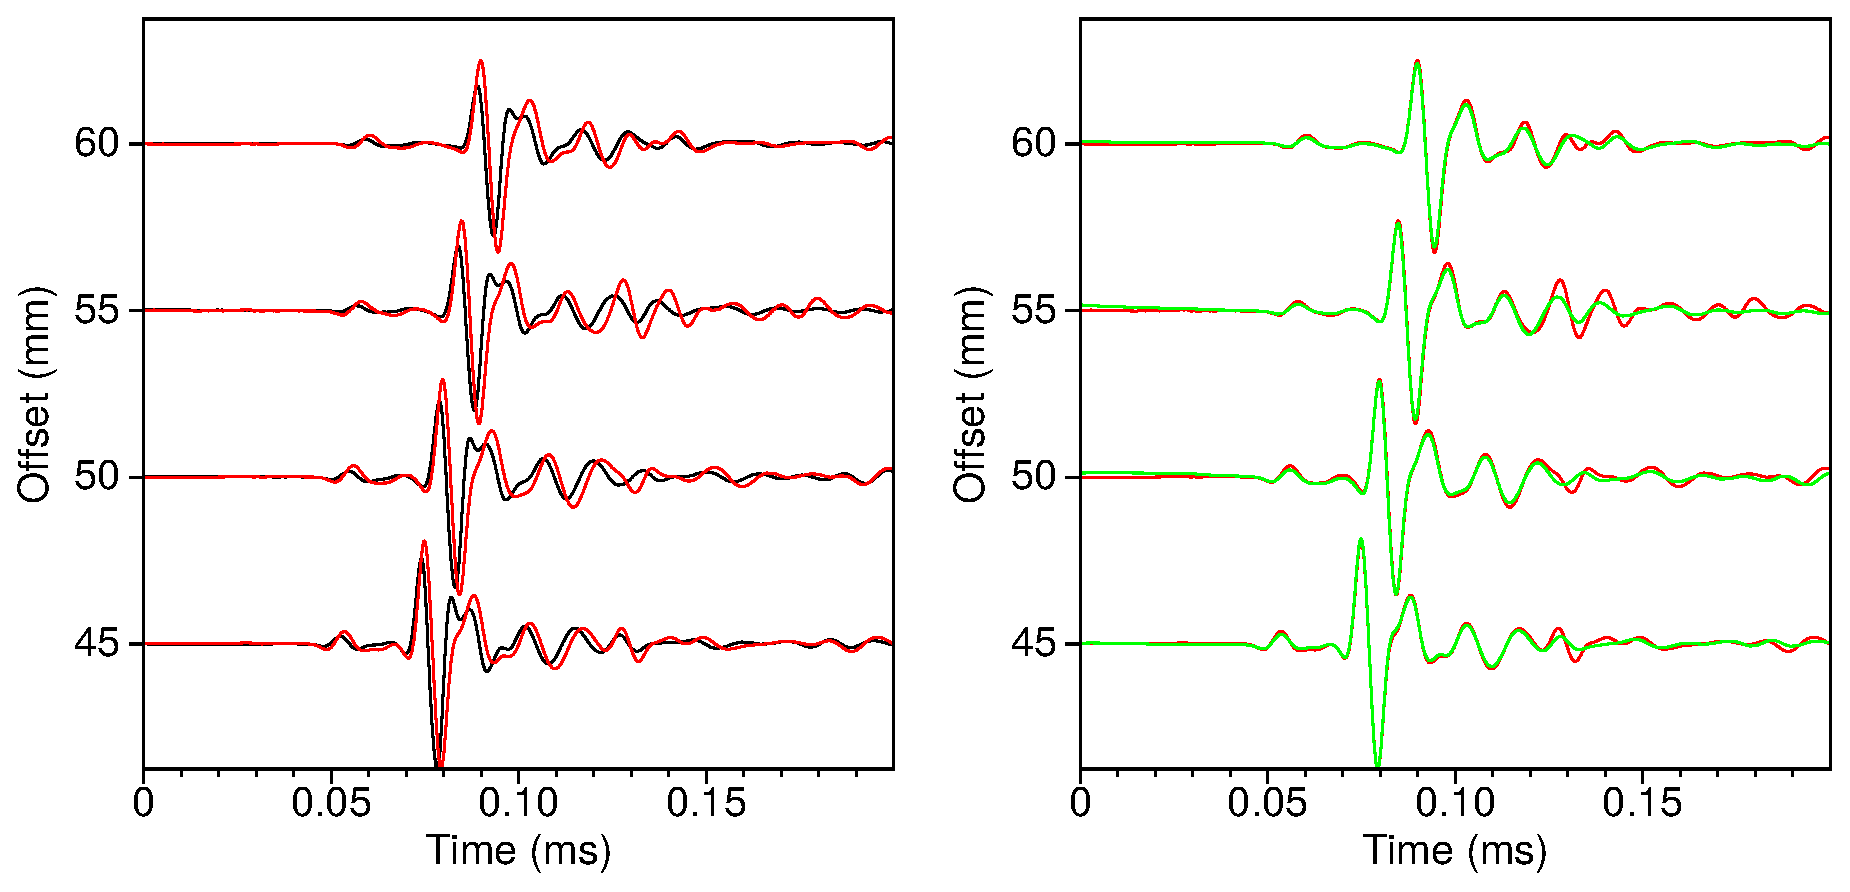
\includegraphics[scale=0.5]{fig/trans2d3d-musc.eps}
	\caption{(a) Comparison between an experimental seismogram for a point-source (red) and for a line source (black), for 50, 55, 60 and 65 mm source-receiver offsets respectively. (b) Comparison between an experimental seismogram for a line-source (black), and a point-source response corrected from geometrical spreading (green) for same source-receiver offsets as (a). \textbf{cc} gives the correlation factor between line-source and point-source responses.}
	\label{panel_amplitude}
\end{figure}

% #### Fig:: panel_srcest_2d_mean
\begin{figure}[!h]
	\centering
	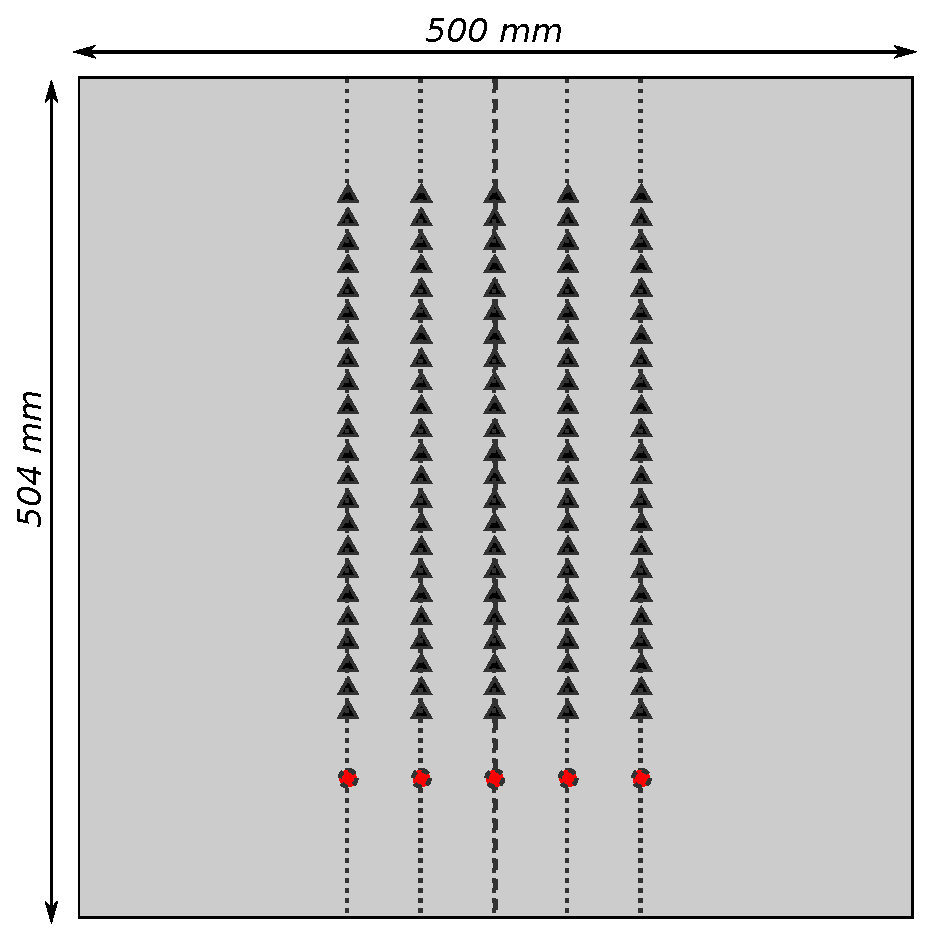
\includegraphics[scale=0.5]{fig/reproducibility_acqui_principle.eps}
	\caption{Schematic representation of the acquisition geometry used to assess the data reproducibility using the MUSC system. Black traingle and red circle represent receivers and sources, respectively.}
	\label{reproducibility_acqui_principle}
\end{figure}

\begin{figure}[!h]
	\centering
	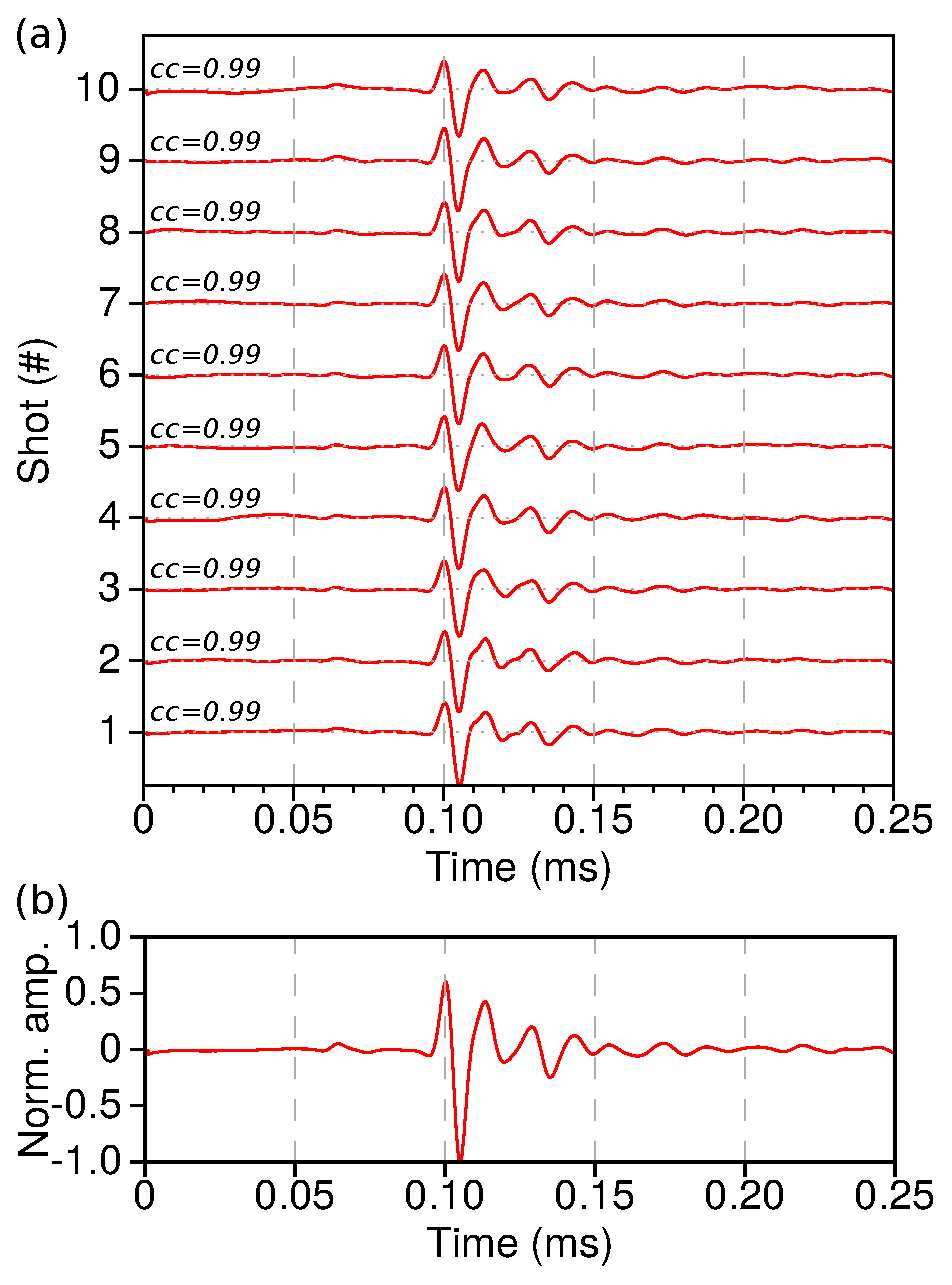
\includegraphics[scale=0.5]{fig/musc_F50_CT.eps}
	\caption{Central trace for each of the ten analogic experiment. \textbf{cc} gives the correlation factor of each central trace with respect to a mean trace.}
	\label{panel_central_traces_cc}
\end{figure}

\begin{figure}[!h]
	\centering
	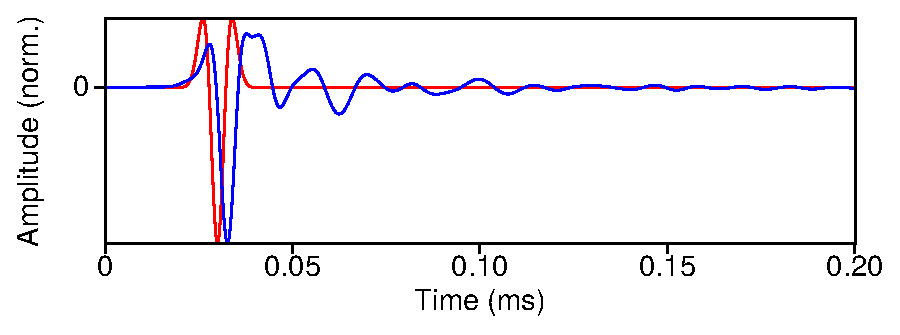
\includegraphics[scale=0.5]{fig/srccomp.eps}
	\caption{Comparison between the theoritical Ricker source send to the transducer and the effective source wavelet injected in the model.}
	\label{srccomp}
\end{figure}

\begin{figure}[!h]
	\centering
	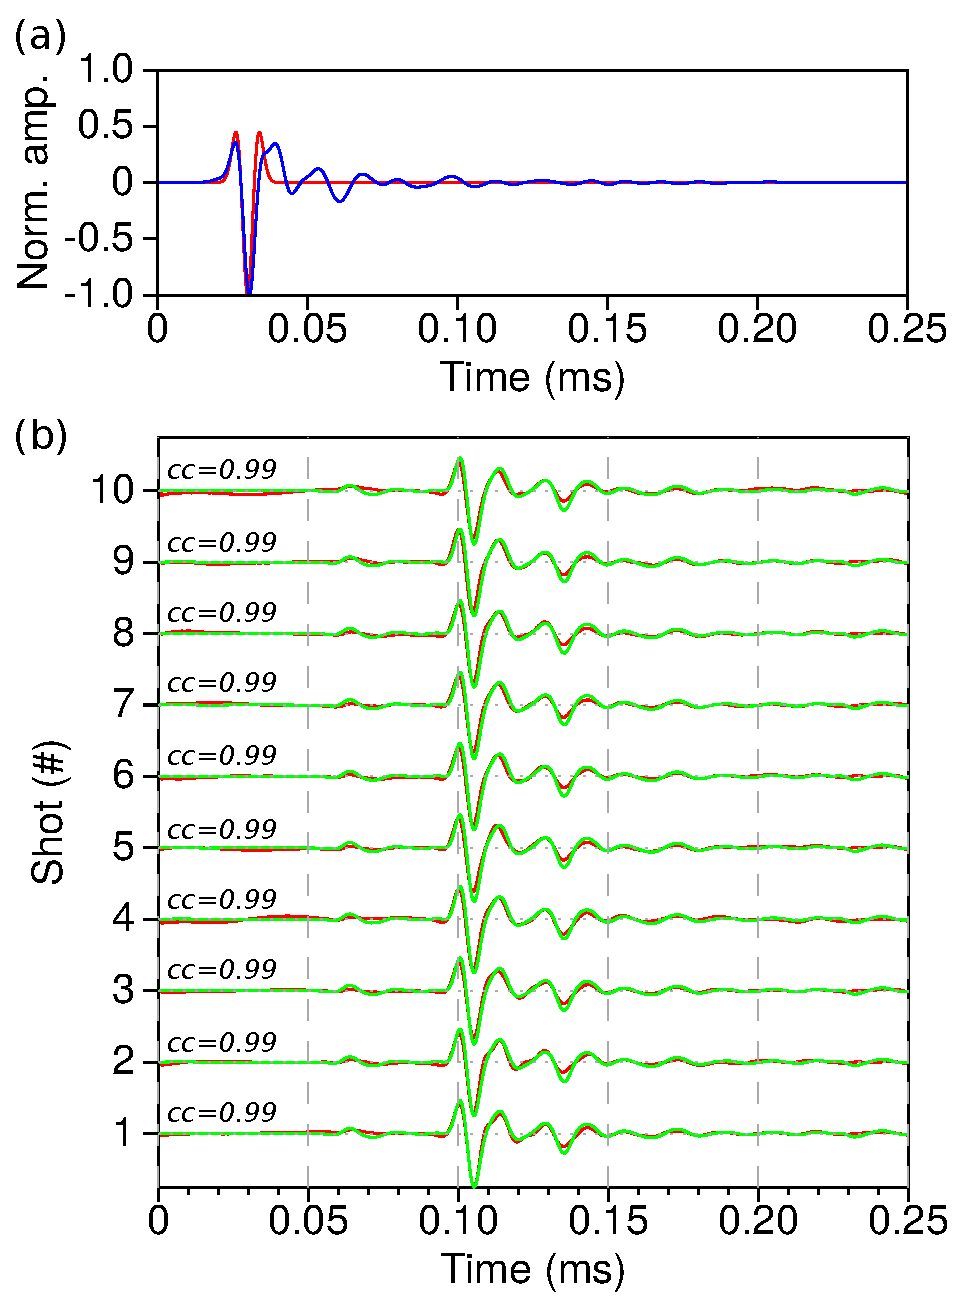
\includegraphics[scale=0.5]{fig/spec_F50_CT_COMP.eps}
	\caption{Comparison between analogic central traces (grey) and numerical traces corrected from the estimated effective source (black) for each experiment. \textbf{cc} gives the correlation coefficient.}
	\label{panel_srcest_2d_mean_comp}
\end{figure}

% #### Fig:: panel_bialt_model
\begin{figure}[!h]
	\centering
	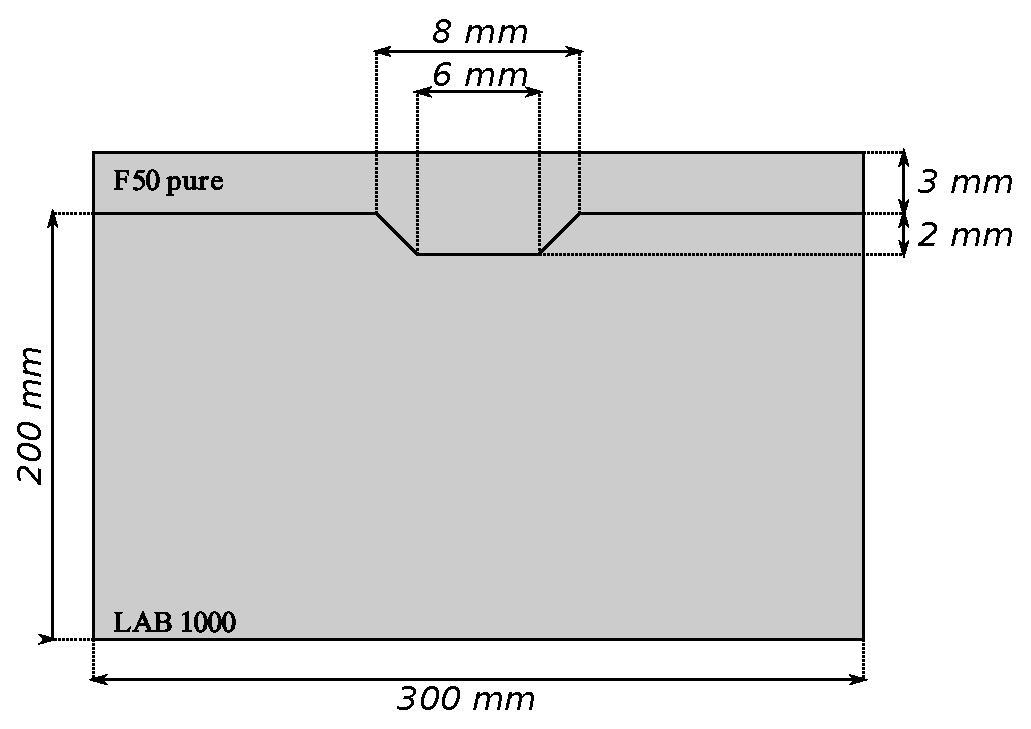
\includegraphics[scale=0.5]{fig/bialt_model.eps}
	\caption{Schematic representation of the so-called \textit{BiAlt} model.}
	\label{panel_bialt_model}
\end{figure}

\begin{figure}[!h]
	\centering
	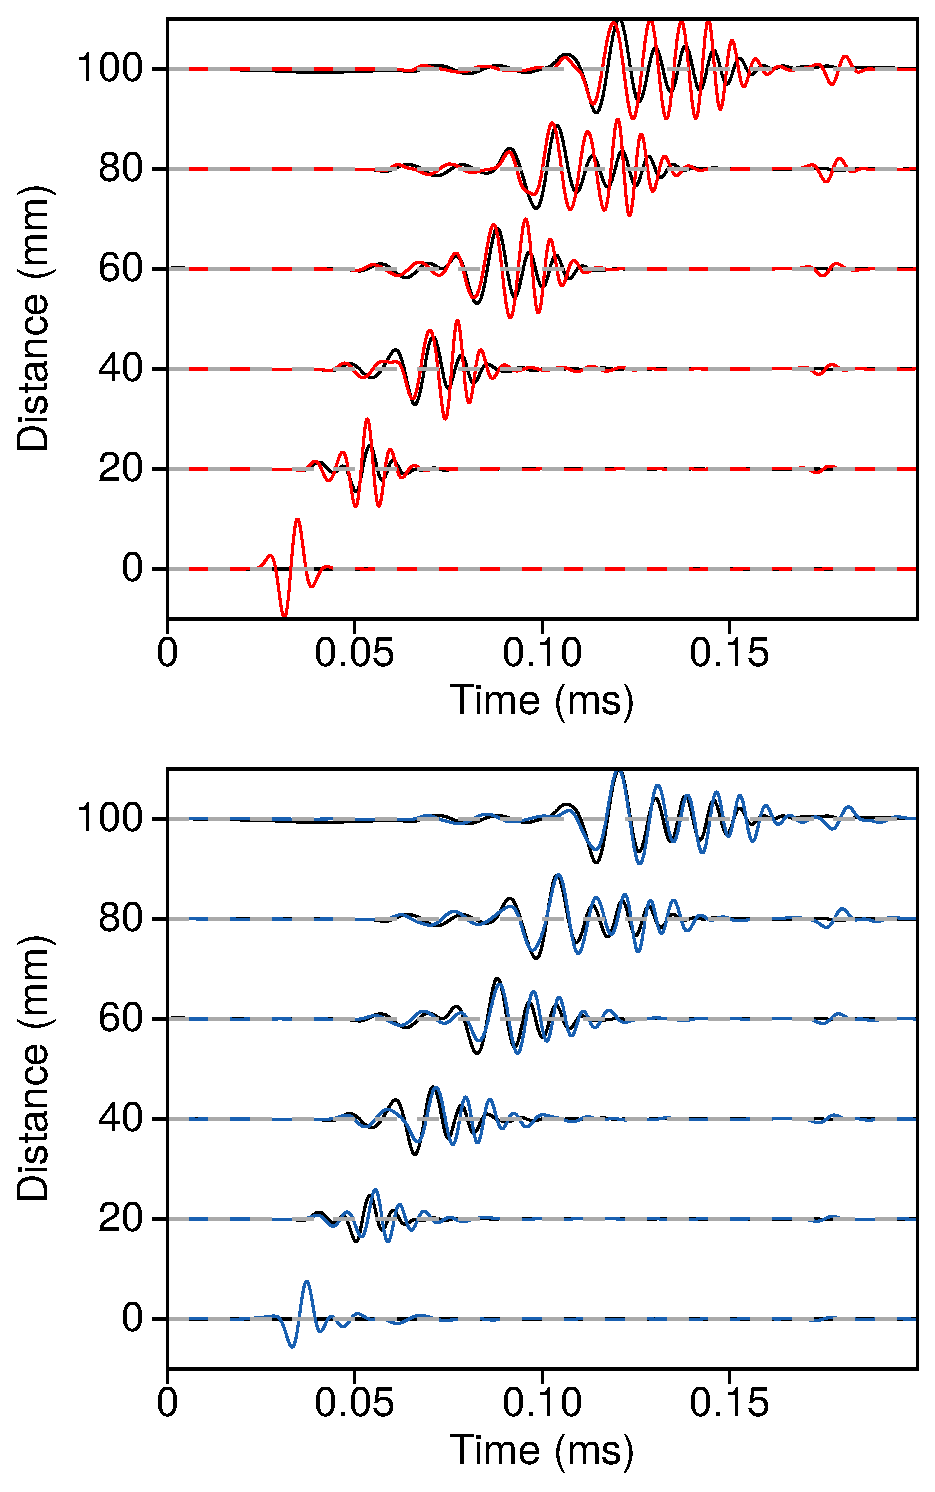
\includegraphics[scale=0.5]{fig/blind-comp-cor.eps}
	\caption{.}
	\label{blind-test}
\end{figure}

\clearpage
\newpage

\subsection*{Tables}

\begin{table}[!ht]
	\centering
	\begin{tabular}{cccccc}
		\hline
		material & $\mathrm{V_{P}\ (m/s)}$ & $\mathrm{V_{S}\ (m/s)}$ & $\mathrm{V_{R}\ (m/s)}$ & $\mathrm{\rho\ (kg/m^{3})}$ & $\mathrm{Q}$ \\
		\hline
		Aluminium & 5630 & 3225 & --   & 2700 & --  \\
		F50 pure  & 2300 & 1030 & 965  & 1300 & 30  \\
		F50 200\% & 2820 & 1425 & 1328 & 1766 & --  \\
		F50 240\% & 2968 & 1496 & 1388 & 1822 & --  \\
		LAB1000   & 2850 & 1400 & 1310 & 1500 & 75  \\
		\hline
	\end{tabular}
	\caption{Physical properties of some materials used to build small scale models. $\mathrm{V_{P}}$, $\mathrm{V_{S}}$ and $\mathrm{V_{R}}$ are the P-wave velocity, S-wave and the Rayleigh wave velocity, respectively. $\rho$ is the density and $\mathrm{Q}$ is the quality factor.}
	\label{epoxy-resin}
\end{table}

\clearpage
\newpage

\begin{table}[!ht]
	\centering
	\begin{tabular}{lcccc}
		\hline
		\qquad & 90 mm & 95 mm & 100 mm & 105 mm \\
		\hline
		$cc1_{init}$  & 0.702 & 0.725 & 0.728 & 0.728 \\
		$rms1_{init}$ & 0.794 & 0.760 & 0.762 & 0.774 \\
		\hline
		$cc1_{final}$  & 0.940 & 0.953 & 0.951 & 0.949 \\
		$rms1_{final}$ & 0.358 & 0.317 & 0.325 & 0.343 \\
		\hline
		\hline
		$cc2_{init}$  & 0.954 & 0.987 & 0.988 & 0.988 \\
		$rms2_{init}$ & 0.304 & 0.162 & 0.155 & 0.154 \\
		\hline
		$cc2_{final}$  & --   & --    & --    & --    \\
		$rms2_{final}$ & --   & --    & --    & --    \\
		\hline
	\end{tabular}
	\caption{.}
	\label{cc-rms}
\end{table}

\clearpage
\newpage 

\section{ACKNOWLEDGMENTS}

\clearpage
\newpage

\bibliographystyle{seg}  % style file is seg.bst
%\bibliography{/media/pageotd/1581-58C8/Work/git-repository//TR-VIBRIS/tail/bibvibris}
\bibliography{bibvibris,bibvibris_Dona,bibvibris-Dona,references}

\end{document}
